\documentclass[11pt,a4paper]{article}
\usepackage[utf8]{inputenc}
\usepackage[german]{babel}
\usepackage{amsmath}
\usepackage{amsfonts}
\usepackage{subfig}
\usepackage{amssymb}
\usepackage{siunitx,physics}
\usepackage{mathtools}
\usepackage{graphicx}
%\usepackage{Here}
\usepackage[version=4]{mhchem}
\usepackage{url}
\usepackage{setspace}
\usepackage[left=2.5cm,right=2.5cm,top=2.5cm,bottom=2cm]{geometry}
[biblography=totocnumbered]
\usepackage{fancyhdr}
\usepackage{scrextend}
\usepackage{hyperref}
\pagenumbering{gobble}

\makeatletter
\newcommand\bigcdot{\mathpalette\bigcdot@{.5}}
\newcommand\bigcdot@[2]{\mathbin{\vcenter{\hbox{\scalebox{#2}{$\m@th#1\bullet$}}}}}
\makeatother

\makeatletter
%\renewcommand*\bib@heading{%
%  \subsection*{}%
%  \@mkboth{\refname}{\refname}}
%\makeatother
\numberwithin{equation}{section}
\numberwithin{figure}{section}

\renewcommand{\labelitemii}{\labelitemfont$\vartriangleright$}
\begin{document}\\
\begin{addmargin}[25pt]{0pt}   
Die langen Polymerketten können an einem Punkt im Kristall enden und dadurch dort einen Punktdefekt verursachen. Andererseits kann in den Ketten die \glqq zick-zack-Form\grqq gebrochen werden. Diesen Defekt nennt man Reneker-Defekt.
\begin{figure}[h]
    \centering
    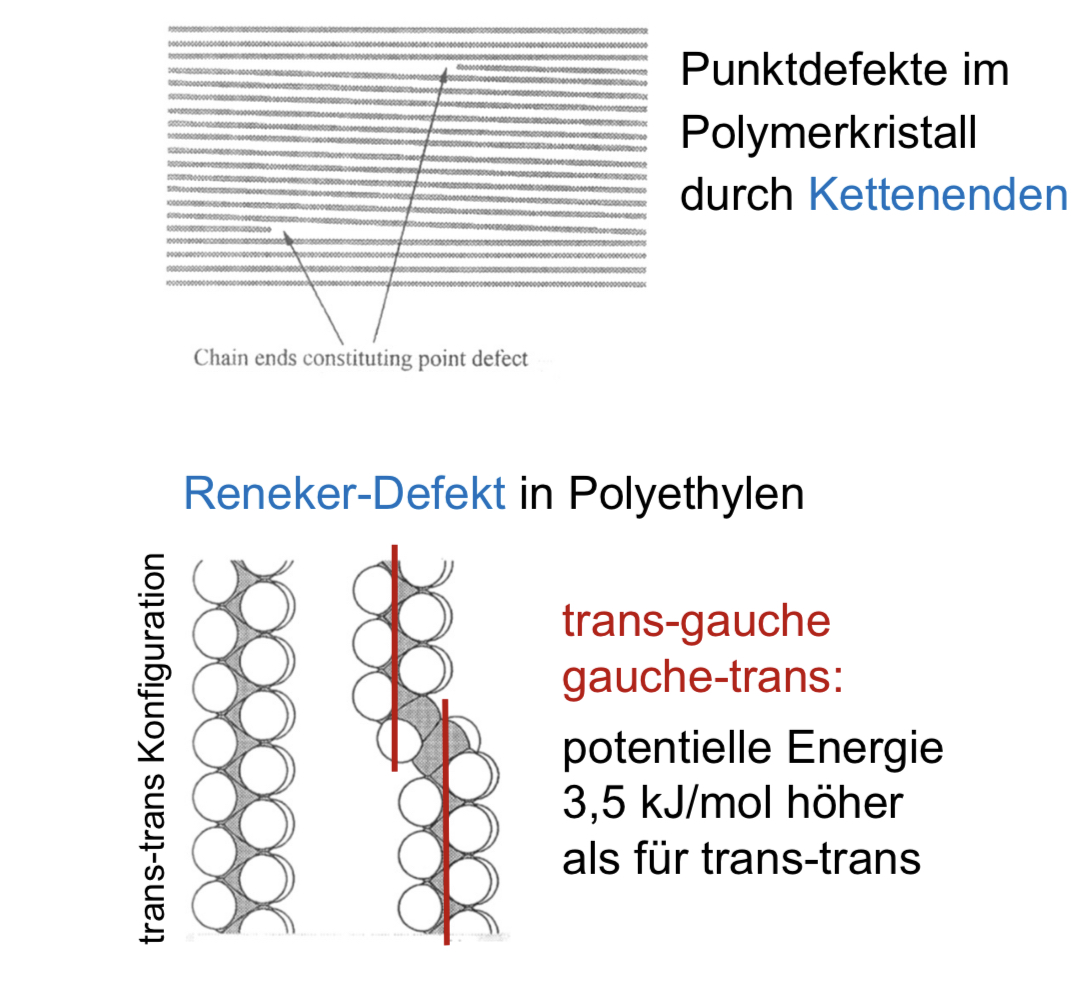
\includegraphics[width = 0.6\textwidth]{images/Materialwissenschaften/Polymerdefekte.jpeg}
    \caption{Die zwei Arten von Defekten in Polymeren. Oben sieht man das unerwartete Ende der Kette und unten ist die spontane Änderung der \glqq zick-zack-Form\grqq dargestellt}
    \label{fig:Polymerdefekte}
\end{figure}
\end{addmargin}

\end{document}